%! Author = fraser
%! Date = 03/04/2021

% Preamble
\documentclass{article}

% Packages
\usepackage{fancyvrb}
\usepackage{pdflscape}
\usepackage{graphicx}
\usepackage{float}
\usepackage[utf8]{inputenc}
\usepackage{xparse}
\usepackage{caption}
\usepackage{subcaption}
\usepackage{geometry}
\usepackage{minted}
\usepackage{amssymb}
\usepackage{tikz}

\usetikzlibrary{arrows,shapes.gates.logic.US,shapes.gates.logic.IEC,calc}
\newcommand{\lnor}{\bar{\hspace*{0.3em}\lor\hspace*{0.2em}}}
\newcommand{\lnand}{\bar{\hspace*{0.3em}\land\hspace*{0.2em}}}
\newcommand{\lxor}{\oplus}
\newcommand{\lxnor}{\hspace*{0.3em}\underbar{\hspace*{-0.3em}\lnor\hspace*{-0.2em}}\hspace*{0.2em}}
\tikzstyle{branch}=[fill,shape=circle,minimum size=3pt,inner sep=0pt]
\newcommand{\size}[2]{{\fontsize{#1}{0}\selectfont#2}}
\newenvironment{sizepar}[2]
{\par\fontsize{#1}{#2}\selectfont}
{\par}

% Document
\begin{document}

    \nocite{*}

    \begin{center}
        \Huge
        CS2002 Week 9 Practical

        \vspace{0.5cm}

        \textbf{Logic}

        \vspace{1cm}
        \LARGE
        3rd April 2021

        \large
        \vspace{1.5cm}

        \textbf{Matriculation Number: 200002548}

        \vspace{0.5cm}

        \textbf{Tutor: Marco Caminati}

    \end{center}

    \vspace*{3cm}

    \tableofcontents

    \newpage
    \section{Introduction}
    The aim of this practical was to gain experience with propositional and digital logic
    through writing truth tables, understanding the equivalence of two different propositional
    formulas and understanding how to represent a formula as a circuit and vice versa.
    \section{Boolean Algebra}
    \begin{enumerate}
        \item $\lnot A \land (B \lor A)$ \\
        $= (\lnot A \land B) \lor (\lnot A \land A)$ \textit{\textbf{\size{7}{(distributivity)}}} \\
        $= (\lnot A \land B) $ \textit{\textbf{\size{7}{(complementation, identity)}}} \\
        $= B \land \lnot A$ \textit{\textbf{\size{7}{(commutativity)}}} \\
        \textbf{The equation holds.} \\ \\

        \item $\lnot(\lnot(\lnot A \lor B) \lor A) \lor A$ \\
        $= ((\lnot A \lor B) \land \lnot A) \lor A$ \textit{\textbf{\size{7}{(de morgan, double negation)}}} \\
        $= (\lnot A) \lor A$ \textit{\textbf{\size{7}{(absorption)}}} \\
        $= T$ \textit{\textbf{\size{7}{(complementation)}}} \\
        \textbf{The equation holds.} \\ \\

        \item $A \land (B \land (\lnot C \land \lnot A))$ \\
        $= (A \land \lnot A) \land \lnot C \land B$ \textit{\textbf{\size{7}{(associativity)}}} \\
        $= F$ \textit{\textbf{\size{7}{(complementation, domination)}}} \\

            \begin{array}{c c c|c c c c|c c}
                A & B & C & \lnot A & \lnot C & \lnot C \land \lnot A & B \land (\lnot C \land \lnot A) & A \land (B \land (\lnot C \land \lnot A)) & B \land \lnot C\\
                \hline
                F & F & F & T & T & T & F & F & F\\
                F & F & T & T & F & F & F & F & F\\
                F & T & F & T & T & T & T & F & T\\
                F & T & T & T & F & F & F & F & F\\
                T & F & F & F & T & F & F & F & F\\
                T & F & T & F & F & F & F & F & F\\
                T & T & F & F & T & F & F & F & T\\
                T & T & T & F & F & F & F & F & F\\
            \end{array} \\ \\
        \textbf{The equation does not hold.} \\ \\

        \item $\lnot(A \lxor (B \land \lnot C))$ \\
        $= \lnot ((A \land \lnot(B \land \lnot C)) \lor (\lnot A \land (B \land \lnot C)))$ \textit{\textbf{\size{7}{($\lxor$ substitution)}}} \\
        $= \lnot(A \land \lnot (B \land \lnot C)) \land \lnot (\lnot A \land B \land \lnot C)$ \textit{\textbf{\size{7}{(de morgan)}}} \\
        $= (\lnot A \lor (B \land \lnot C)) \land (A \lor \lnot B \lor C)$ \textit{\textbf{\size{7}{(de morgan, double negation)}}} \\
        $= (\lnot A \land (A \lor \lnot B \lor C)) \lor (B \land \lnot C \land (A \lor \lnot B \lor C))$ \textit{\textbf{\size{7}{(distributivity)}}} \\
        $= (\lnot A \land A) \lor (\lnot A \land \lnot B) \lor (\lnot A \land C) \lor (B \land \lnot C \land A) \lor (B \land \lnot C \land \lnot B) \lor (B \land \lnot C \land C)$ \textit{\textbf{\size{7}{(distributivity)}}} \\
        $= (\lnot A \land \lnot B) \lor (\lnot A \land C) \lor (B \land \lnot C \land A)$ \textit{\textbf{\size{7}{(complementation, identity)}}} \\

            \begin{array}{c c c|c c c c c c c}
                A & B & C & \lnot A & \lnot B & \lnot C & \lnot A \land \lnot B & \lnot A \land C & B \land \lnot C \land A & A \land \lnot B \\
                \hline
                F & F & F & T & T & T & T & F & F & F\\
                F & F & T & T & T & F & T & T & F & F\\
                F & T & F & T & F & T & F & F & F & F\\
                F & T & T & T & F & F & F & T & F & F\\
                T & F & F & F & T & T & F & F & F & T\\
                T & F & T & F & T & F & F & F & F & T\\
                T & T & F & F & F & T & F & F & T & F\\
                T & T & T & F & F & F & F & F & F & F\\
            \end{array} \\ \\

            \begin{array}{c c}
                (\lnot A \land \lnot B) \lor (\lnot A \land C) \lor (B \land \lnot C \land A) & (A \land \lnot B) \lor C\\
                \hline
                T & F\\
                T & T\\
                F & F\\
                T & T\\
                F & T\\
                F & T\\
                T & F\\
                F & T\\
            \end{array} \\ \\
        \textbf{The equation does not hold.} \\ \\

        \item $(A \to (B \land C)) \lor \lnot(A \land C)$ \\
        $= \lnot A \lor (B \land C) \lor \lnot A \lor \lnot C$ \textit{\textbf{\size{7}{($\to$ substitution, de morgan)}}} \\
        $= \lnot A \lor (B \land C) \lor \lnot C$ \textit{\textbf{\size{7}{(idempotent)}}} \\
        $= \lnot A \lor (\lnot C \lor B) \land (\lnot C \lor C)$ \textit{\textbf{\size{7}{(distributivity)}}} \\
        $= \lnot C \lor B \lor \lnot A $ \textit{\textbf{\size{7}{(complementation, identity, commutativity)}}} \\
        \textbf{The equation holds.} \\ \\
    \end{enumerate}

    \section{Formula to Circuit}
    \begin{enumerate}
        \item $(\lnot A \lor \lnot B) \lxor (C \lor A)$ \\
        $= ((\lnot A \lor \lnot B) \land \lnot (C \lor A)) \lor (\lnot (\lnot A \lor \lnot B) \land (C \lor A))$ \textit{\textbf{\size{7}{($\lxor$ substitution)}}} \\
        $=  ((\lnot A \lor \lnot B) \land \lnot C \land \lnot A) \lor (A \land B \land (C \lor A))$ \textit{\textbf{\size{7}{(de morgan, double negation)}}} \\
        $= (\lnot C \land \lnot A \land \lnot A) \lor (\lnot C \land \lnot A \land \lnot B) \lor (A \land B \land (C \lor A))$ \textit{\textbf{\size{7}{(distributivity)}}} \\
        $= (\lnot C \land \lnot A) \lor (\lnot C \land \lnot A \land \lnot B) \lor (A \land B \land (C \lor A))$ \textit{\textbf{\size{7}{(idempotent)}}} \\
        $= (\lnot C \land \lnot A) \lor (A \land B \land (C \lor A))$ \textit{\textbf{\size{7}{(absorption)}}} \\
        $= (\lnot C \land \lnot A) \lor (A \land B \land C) \lor (A \land B \land A)$ \textit{\textbf{\size{7}{(distributivity)}}} \\
        $= (\lnot C \land \lnot A) \lor (A \land B \land C) \lor (A \land B)$ \textit{\textbf{\size{7}{(idempotent)}}} \\
        $= (\lnot A \land \lnot C) \lor (A \land B)$ \textit{\textbf{\size{7}{(absorption, commutativity)}}} \\
        $= (A \lnor C) \lor (A \land B) $ \textit{\textbf{\size{7}{($\lnor$ substitution)}}} \\

        \begin{array}{c c c c|c c}
            A & C & \lnot A & \lnot C & \lnot A \land \lnot C & A \lnor C \\
            \hline
            F & F & T & T & T & T\\
            F & T & T & F & F & F\\
            T & F & F & T & F & F\\
            T & T & F & F & F & F\\
        \end{array} \\ \\

        \begin{tikzpicture}
            \node (A) at (0,2) {A};
            \node (B) at (0,1) {B};
            \node (C) at (0,0) {C};
            \node[and gate US, draw] at (1.5,1.5) (AND1) {};
            \node[nor gate US, draw] at (1.5,0.5) (NOR1) {};
            \node[or gate US, draw] at (3,1) (OR1) {};

            \draw (A) -| ([xshift=-0.75cm]AND1.input 1) node[branch] -| ([xshift=-0.5cm]AND1.input 1) -- (AND1.input 1);
            \draw (B) -| ([xshift=-0.5cm]AND1.input 2) -- (AND1.input 2);
            \draw (C) -| ([xshift=-0.5cm]NOR1.input 2) -- (NOR1.input 2);
            \draw ([xshift=-0.75cm]AND1.input 1) |- ([xshift=-0.75cm]NOR1.input 1) -- (NOR1.input 1);
            \draw (AND1.output) -- ([xshift=0.5cm]AND1.output) |- (OR1.input 1);
            \draw (NOR1.output) -- ([xshift=0.5cm]NOR1.output) |- (OR1.input 2);
            \draw (OR1.output) -- ([xshift=0.5cm]OR1.output);
        \end{tikzpicture} \\ Gate Depth: 2 \\ \\ This is the minimum number of gates possible for this circuit when constrained to using $\left\{\lnot, \lor, \land, \lnor, \lnand, \lxor \right\}$.
        When all 16 variants of logical 2-way gates are allowed all possible types of behaviour is defined when combining two inputs to produce some output.
        Therefore when given 3 inputs these can be combined into one output with the desired behaviour using only two logic gates.
        However due to being constrained to using only 5 2-way logic gates and a NOT gate, this is not always possible.
        Therefore sometimes a combination of these chosen gates is needed to produce the intended behaviour.
        In the circuit above the defined behaviour is unable to be produced with only two of the gates we are constrained to, so a further gate is needed.
        However while this leads to an increase in the total number of gates used, the gate depth will still remain the same as the extra gate can be placed in parallel.\\ \\

        \item $\lnot((A \lor B) \land \lnot(A \lor C)) \lxor C$ \\
        $= (\lnot (A \lor B)\lor A \lor C) \lxor C$ \textit{\textbf{\size{7}{(de morgan)}}} \\
        $= ((\lnot A \land \lnot B) \lor A \lor C) \lxor C$ \textit{\textbf{\size{7}{(de morgan)}}} \\
        $= ((A \lor C \lor \lnot A) \land (A \lor C \lor \lnot B)) \lxor C$ \textit{\textbf{\size{7}{(distributivity)}}} \\
        $= (A \lor \lnot B \lor C) \lxor C$ \textit{\textbf{\size{7}{(complementation, identity, commutativity)}}} \\
        $= ((A \lor \lnot B \lor C) \land \lnot C) \lor (\lnot (A \lor \lnot B \lor C) \land C)$ \textit{\textbf{\size{7}{($\lxor$ substitution)}}} \\
        $= ((A \lor \lnot B \lor C) \land \lnot C) \lor (\lnot A \land B \land \lnot C \land C)$ \textit{\textbf{\size{7}{(de morgan)}}} \\
        $= ((A \lor \lnot B \lor C) \land \lnot C)$ \textit{\textbf{\size{7}{(complementation, domination, identity)}}} \\
        $= (A \land \lnot C) \lor (\lnot B \land \lnot C) \lor (C \land \lnot C)$ \textit{\textbf{\size{7}{(distributivity)}}} \\
        $= (A \land \lnot C) \lor (\lnot B \land \lnot C)$ \textit{\textbf{\size{7}{(complementation, identity)}}} \\
        $= (A \lor \lnot B) \land \lnot C$ \textit{\textbf{\size{7}{(distributivity, commutativity)}}} \\
        $= (\lnot A \land B) \lnor C$ \textit{\textbf{\size{7}{($\lnor$ substitution, de morgan, double negation)}}} \\
        $= (A \lnor \lnot B) \lnor C$ \textit{\textbf{\size{7}{($\lnor$ substitution, double negation)}}} \\

        \begin{array}{c c c|c c c c|c c}
            A & B & C & \lnot B & \lnot C & A \lor \lnot B & A \lnor \lnot B & (A \lor \lnot B) \land \lnot C & (A \lnor \lnot B) \lnor C \\
            \hline
            F & F & F & T & T & T & F & T & T\\
            F & F & T & T & F & T & F & F & F\\
            F & T & F & F & T & F & T & F & F\\
            F & T & T & F & F & F & T & F & F\\
            T & F & F & T & T & T & F & T & T\\
            T & F & T & T & F & T & F & F & F\\
            T & T & F & F & T & T & F & T & T\\
            T & T & T & F & F & T & F & F & F\\
        \end{array} \\ \\

        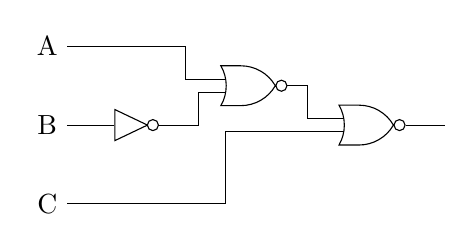
\begin{tikzpicture}
            \node (A) at (0,2) {A};
            \node (B) at (0,1) {B};
            \node (C) at (0,0) {C};
            \node[not gate US, draw] at (1,1) (NOT1) {};
            \node[nor gate US, draw] at (2.5,1.5) (NOR1) {};
            \node[nor gate US, draw] at (4,1) (NOR2) {};

            \draw (B) -- (NOT1.input);
            \draw (A) -| ([xshift=-0.5cm]NOR1.input 1) -| (NOR1.input 1);
            \draw (NOT1.output) -- ([xshift=0.5cm]NOT1.output) |- (NOR1.input 2);
            \draw (NOR1.output) -- ([xshift=0.25cm]NOR1.output) |- (NOR2.input 1);
            \draw (C) -| ([xshift=-1.5cm]NOR2.input 2) -| (NOR2.input 2);
            \draw (NOR2.output) -- ([xshift=0.5cm]NOR2.output);
        \end{tikzpicture}\\ Gate Depth: 3 \\ \\ This circuit is also three inputs to one output and so follows the same logic described above.
        However in the behavior defined by this circuit and the constraints on the types of logic gates that can be used an extra NOT gate is needed.
        This will increase the gate depth since a NOT gate does not combine two inputs into one output, so at most a further 2 gates are required to combine the three inputs to an output.
        If all 2-way gates where allowed then the circuit could be built using the $\lnot A \land B$ equivalent gate, and would reduce the gate depth to 2 since the NOT gate would be no longer required.\\ \\

        \item $A \leftrightarrow B$ \\
        $= (A \to B) \land (B \to A)$ \textit{\textbf{\size{7}{($\leftrightarrow$ substitution)}}} \\
        $= (\lnot A \lor B) \land (\lnot B \lor A)$ \textit{\textbf{\size{7}{($\rightarrow$ substitution)}}} \\
        $= \lnot(A \lxor B)$ \textit{\textbf{\size{7}{($\lxor$ substitution)}}} \\

        \begin{array}{c c|c c c c c|c c}
            A & B & \lnot A & \lnot B & \lnot A \lor B & \lnot B \lor A & A \lxor B & (\lnot A \lor B) \land (\lnot B \lor A) & \lnot(A \lxor B) \\
            \hline
            F & F & T & T & T & T & F & T & T \\
            F & T & T & F & T & F & T & F & F \\
            T & F & F & T & F & T & T & F & F \\
            T & T & F & F & T & T & F & T & T \\
        \end{array} \\ \\

        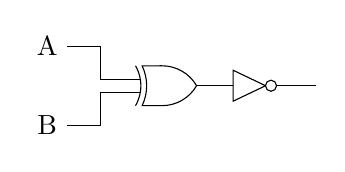
\begin{tikzpicture}
            \node (A) at (0,1) {A};
            \node (B) at (0,0) {B};
            \node[xor gate US, draw] at (1.5,0.5) (XOR1) {};
            \node[not gate US, draw] at (2.5,0.5) (NOT1) {};

            \draw (A) -| ([xshift=-0.5cm]XOR1.input 1) -| (XOR1.input 1);
            \draw (B) -| ([xshift=-0.5cm]XOR1.input 2) -| (XOR1.input 2);
            \draw (XOR1.output) -- (NOT1.input);
            \draw (NOT1.output) -- ([xshift=0.5cm]NOT1.output);
        \end{tikzpicture}\\ Gate Depth: 2 \\ \\ This circuit only needs to combine two gates to one output, however once again because of the logic gate constraints two gates had to be used to obtain the desired behaviour.
        Specifically an extra NOT gate was required after XOR since XNOR gates where not part of the constraint.
        This increases the gate depth and total number of gates in the circuit to 2. \\ \\
    \end{enumerate}

    \section{Circuit to CNF}
    \begin{enumerate}
        \item $(B\lnand A) \lor (\lnot A \lxor C)$ \\
        $= \lnot(B \land A) \lor ((\lnot A \lor C) \land (A \lor \lnot C))$  \textit{\textbf{\size{7}{($\lxor$ substitution, $\lnand$ substitution)}}} \\
        $= \lnot B \lor \lnot A \lor ((\lnot A \lor C) \land (A \lor \lnot C))$ \textit{\textbf{\size{7}{(de morgan)}}} \\
        $= \lnot B \lor \lnot A \lor (\lnot A \land (\lnot A \lor C)) \lor (C \land (A \lor \lnot C))$ \textit{\textbf{\size{7}{(distributivity)}}} \\
        $= \lnot B \lor \lnot A \lor (C \land (A \lor \lnot C))$ \textit{\textbf{\size{7}{(absorption)}}} \\
        $= \lnot B \lor \lnot A \lor (C \land A) \lor (C \land \lnot C)$ \textit{\textbf{\size{7}{(distributivity)}}} \\
        $= \lnot B \lor \lnot A \lor (C \land A)$ \textit{\textbf{\size{7}{(complementation, identity)}}} \\
        $= (\lnot B \lor \lnot A \lor C) \land (\lnot B \lor \lnot A \land A)$ \textit{\textbf{\size{7}{(distributivity)}}} \\
        $= \lnot A \lor \lnot B \lor C$ \textit{\textbf{\size{7}{(complementation, identity, commutativity)}}} \\ \\

        \item $((A \land B) \lor \lnot A) \lnand A$ \\
        $= \lnot(((A \land B) \lor \lnot A) \land A)$ \textit{\textbf{\size{7}{($\lnand$ substitution)}}} \\
        $= \lnot((A \land B) \lor \lnot A) \lor \lnot A$ \textit{\textbf{\size{7}{(de morgan)}}} \\
        $= ((\lnot A \lor \lnot B) \land A) \lor \lnot A$ \textit{\textbf{\size{7}{(de morgan, double negation)}}} \\
        $= (A \land \lnot A) \lor (A \land \lnot B) \lor \lnot A$ \textit{\textbf{\size{7}{(distributivity)}}} \\
        $= (A \land \lnot B) \lor \lnot A$ \textit{\textbf{\size{7}{(complementation, identity)}}} \\
        $= (\lnot A \lor A) \land (\lnot A \lor \lnot B)$ \textit{\textbf{\size{7}{(distributivity)}}} \\
        $= \lnot A \lor \lnot B$ \textit{\textbf{\size{7}{(complementation, identity)}}} \\

        \item $((A \lnand B) \lor A) \lor ((A \lnand B) \land B)$ \\
        $= \lnot(A \land B) \lor A \lor (\lnot(A \land B) \land B)$ \textit{\textbf{\size{7}{($\lnand$ substitution)}}} \\
        $= A \lor \lnot A \lor \lnot B \lor ((\lnot A \lor \lnot B) \land B)$ \textit{\textbf{\size{7}{(de morgan, commutativity)}}} \\
        $= T$ \textit{\textbf{\size{7}{(complementation, domination)}}} \\
    \end{enumerate}

    \section{Additional Proofs}
    These proofs are included to show that substitutions made throughout the practical are logically correct. \\

    \noindent $(A \lnor B) \iff \lnot(A \lor B) \iff (\lnot A \land \lnot B)$ \\ \\
    \begin{array}{c c|c c c|c c c}
        A & B & \lnot A & \lnot B & A \lor B & \lnot A \land \lnot B & \lnot (A \lor B) & A \lnor B \\
        \hline
        F & F & T & T & F & T & T & T \\
        F & T & T & F & T & F & F & F \\
        T & F & F & T & T & F & F & F \\
        T & T & F & F & T & F & F & F \\
    \end{array} \\ \\

    \noindent $(A \lnand B) \iff \lnot(A \land B) \iff (\lnot A \lor \lnot B)$ \\ \\
    \begin{array}{c c|c c c|c c c}
        A & B & \lnot A & \lnot B & A \land B & \lnot A \lor \lnot B & \lnot (A \land B) & A \lnand B \\
        \hline
        F & F & T & T & F & T & T & T \\
        F & T & T & F & F & T & T & T \\
        T & F & F & T & F & T & T & T \\
        T & T & F & F & T & F & F & F \\
    \end{array} \\ \\

    \noindent $(A \iff B) \iff (A \to B) \land (B \to A)$ \\ \\
    \begin{array}{c c|c c|c c}
        A & B & A \to B & B \to A & (A \to B) \land (B \to A) & A \iff B \\
        \hline
        F & F & T & T & T & T \\
        F & T & T & F & F & F \\
        T & F & F & T & F & F \\
        T & T & T & T & T & T \\
    \end{array} \\ \\

    \noindent $(A \to B) \iff (\lnot A \lor B)$ \\ \\
    \begin{array}{c c|c|c c}
        A & B & \lnot A & A \to B & \lnot A \lor B\\
        \hline
        F & F & T & T & T \\
        F & T & T & T & T \\
        T & F & F & F & F \\
        T & T & F & T & T \\
    \end{array} \\ \\
    
    \noindent $(A \lxor B) \iff (\lnot A \land B) \lor (\lnot B \land A)$ \\ \\
    \begin{array}{c c|c c c c|c c}
        A & B & \lnot A & \lnot B & \lnot A \land B & \lnot B \land A & A \lxor B & (\lnot A \land B) \lor (\lnot B \land A) \\
        \hline
        F & F & T & T & F & F & F & F \\
        F & T & T & F & T & F & T & T \\
        T & F & F & T & F & T & T & T \\
        T & T & F & F & F & F & F & F \\
    \end{array} \\ \\

    \section{Conclusion}
    From this practical I have developed my ability to simplify propositional logic to produce more efficient logical circuits with a smaller total number of gates and gate depths.
    I have also learned how to convert any logic formula to conjunctive normal form (CNF).
    Moreover I have learned how constricting the types of logic gates in a circuit can cause the number of gates in the circuit and gate depth be larger than its counterparts using all 16, 2-way logic gates.

    \begin{thebibliography}{10}
        \bibitem{numeric}
        Wolfram, \textit{XOR}, 26-03-2021, accessed 05-04-2021, \\\texttt{https://mathworld.wolfram.com/XOR.html}
        \bibitem{numeric}
        Scott H, \textit{A quick way to remember NAND \& NOR logic?}, 01-11-2011, accessed 05-04-2021, \\\texttt{https://electronics.stackexchange.com/a/21653}
    \end{thebibliography}


\end{document}